\documentclass{standalone}

\usepackage[OT1]{fontenc}
\renewcommand*\familydefault{\sfdefault}
\usepackage{helvet,sfmath}
\usepackage{siunitx}

\usepackage{tikz}
\usetikzlibrary{arrows,calc,patterns}
% \usetikzlibrary{intersections, calc, arrows.meta}
\usepackage{tikz,tkz-euclide}

\begin{document}

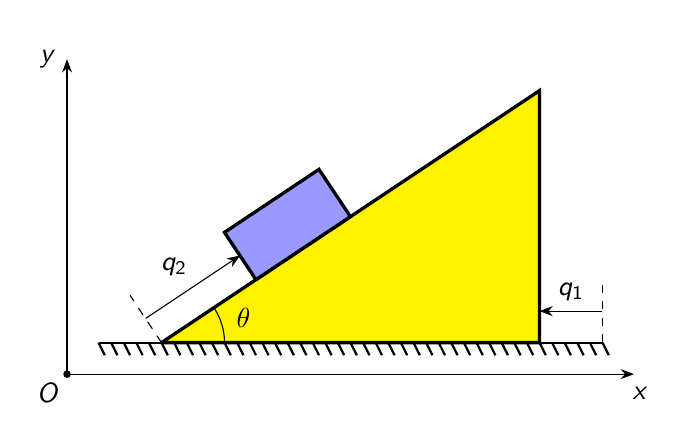
\begin{tikzpicture}[scale=0.8]
    %%Background
    \draw[draw=none] (0,-1) rectangle (10,5);
    
    %% Wedge
    \draw[thick] (1,0) to (9,0);
    \foreach \x in {1,1.2,...,9}
    {
    \draw[thick] (\x,0) to (\x+0.1,-0.2);
    }
    \draw[fill=yellow, very thick] (2,0) to (8,0) to (8,4) to (2,0);
    \draw[fill=blue!40, very thick] (3.5,1) to (5,2) to (4.5,2.75) to (3,1.75) to (3.5,1);

    %% Coordinate
    \draw[-Stealth] (0.5,-0.5) to (9.5,-0.5);
    \draw[-Stealth] (0.5,-0.5) to (0.5,4.5);
    \draw[fill=black] (0.5,-0.5) circle (0.05);
    \draw
    (0.2,-0.8) node{\(O\)}
    (9.6,-0.8) node{\(x\)}
    (0.2,4.5) node{\(y\)}
    ;

    \draw[dashed] (2,0) to (1.5,0.75);
    \draw[-Stealth] (1.75,0.385) to (3.25,1.385);
    \draw[dashed] (9,0) to (9,1);
    \draw[-Stealth] (9,0.5) to (8,0.5);

    \draw
    (8.5,0.8) node{\(q_1\)}
    (2.2,1.2) node{\(q_2\)}
    ;

    \draw (3,0) arc (0:33:1);
    \draw (3.3,0.4) node{\(\theta\)};
    
\end{tikzpicture}

\end{document}
